\documentclass{VUMIFPSkursinis}
\usepackage{algorithmicx}
\usepackage{algorithm}
\usepackage{algpseudocode}
\usepackage{amsfonts}
\usepackage{amsmath}
\usepackage{bm}
\usepackage{caption}
\usepackage{color}
\usepackage{float}
\usepackage{graphicx}
\usepackage{listings}
\usepackage{subfig}
\usepackage{wrapfig}
% \usepackage{lithuanian}
\usepackage{longtable}
\usepackage{xcolor}


\usepackage{enumitem}
%PAKEISTA, tarpai tarp sąrašo elementų
\setitemize{noitemsep,topsep=0pt,parsep=0pt,partopsep=0pt}
\setenumerate{noitemsep,topsep=0pt,parsep=0pt,partopsep=0pt}

% Titulinio aprašas
\university{Vilniaus universitetas}
\faculty{Matematikos ir informatikos fakultetas}
\department{Programų sistemų katedra}
\papertype{Kursinis darbas}
\title{Rodiklių duomenų kaupimas, transformavimas ir analizė, naudojant srautinį duomenų apdorojimą}
\titleineng{Indicator Data Collection, Transformation and Analysis Using Stream Processing}
\status{3 kurso 5 grupės studentas}
\author{Vytautas Žilinas}
\supervisor{lekt. Andrius Adamonis}
\date{Vilnius – \the\year}

% Nustatymai
% \setmainfont{Palemonas}   % Pakeisti teksto šriftą į Palemonas (turi būti įdiegtas sistemoje)
%\bibliography{bibliografija}
%\documentclass{article}
\usepackage[backend=biber]{biblatex}
\addbibresource{bibliografija.bib}
\begin{document}
	
% PAKEISTA	
\maketitle
\cleardoublepage\pagenumbering{arabic}
\setcounter{page}{2}

%TURINYS
\tableofcontents

\sectionnonum{Įvadas}

    Šiame darbe rodiklių duomenys yra apibrėžti kaip didelių duomenų tipas. Šiuos duomenis galima transformuoti, analizuoti ir grupuoti pagal pasirinktus rodiklius, 
pavyzdžiui: bazinė mėnesio alga, mirusiųjų skaičius pagal mirties priežastis, krituliai per metus. 
Rodiklių duomenų bazės pasižymi tuo, kad duomenys į jas patenka iš daug skirtingų tiekėjų, o patekimo laikas tarp
tiekėjų nėra sinchronizuojamas. Tuo tarpų suagreguotą informaciją vartotojai gali užklausti irgi bet kurio metu. \par
Lietuvoje rodiklių duomenų bazės pavyzdys yra ,,Lietuvos statistikos departamento" duomenų bazė, kurioje užklausas galima vykdyti
\url{https://osp.stat.gov.lt/statistiniu-rodikliu-analize#/} puslapyje, kuris leidžia ieškoti duomenis apdorotus pagal vieną arba kelis rodiklius. 
Kitas pavyzdys yra ,,DataBank" \url{http://databank.worldbank.org} - pasaulinio lygio rodiklių duomenų bazių rinkinys, turintis 69 skirtingas 
duomenų bazes, pavyzdžiui - ,,World development indicators", ,,Gander statistics" \cite{databank-stats}. \par
Rodiklių duomenims galima pritaikyti dalį didelių duomenų charakteristikų ir apsibrėžti, kurios iš jų mums sukelia daugiausiai iššūkių.
Didelių duomenų iššūkiai yra apibrėžti Gartner's Doug Laney pristatytu 3V modeliu \cite{laney20013d},
kuris buvo papildytas Bernard Marr iki 5V modelio \cite{marr2014big}:
\begin{itemize}
    \item Tūris (angl. Volume). Apibrėžia generuojamų duomenų kiekius. Didelių duomenų atveju yra šnekama apie duomenų kiekius, kuriuos yra sudėtinga arba neįmanoma saugoti 
    ir analizuoti centralizuotomis duomenų bazių valdymo sistemomis. Rodiklių duomenų kiekiai nesudaro problemos saugojant, tačiau problema yra rodiklių duomenų analizė, 
    kadangi tuos pačius duomenis reikia apdoroti pagal neribotą kiekį skirtingų rodiklių.
    \item Greitis (angl. Velocity). Apibrėžia greitį, kuriuo nauji duomenys yra generuojami. Rodiklių duomenų atveju, tai yra svarbu, kadangi nauji duomenys, kurie gali 
    tikti skirtingiems rodikliams, yra generuojami pastoviai.
    \item Įvairovė (angl. Variety). Apibrėžia duomenų tipus. Duomenys gali būti: struktūrizuoti, nestruktūrizuoti arba dalinai struktūrizuoti \cite{zikopoulos2011understanding}. 
    Rodiklių duomenys yra struktūrizuoti, todėl tai nėra aktualus iššūkis.
    \item Tikrumas (angl. Veracity). Apibrėžia duomenų teisingumą ir kokybę. Pavyzdžiui, jeigu būtų analizuojamas ,,Twitter" socialinio tinklo žinučių turinys, būtų gauta
    daug gramatikos klaidų, naujadarų, slengo. 
    Statistinio departamento atveju duomenys visada, kiek įmanoma, bus tvarkingi, kadangi tai yra duomenys surinkti iš dokumentų ir apklausų, o ne laisvai įvedami.
    \item Vertė (angl. Value). Apibrėžia duomenų ekonominę vertę. Rodiklių duomenys yra vertingi įstaigoms, nes tos įstaigos užsiima tik rodiklių duomenų kaupimų ir analizė, iš techninės pusės
    ši charakteristika yra svarbi, nes duomenų apdorojimo ir kaupimo sprendimai daro įtaką įstaigoms, kaupiančioms rodiklių duomenis, veiklai. 
    Todėl šie apdoroti duomenys turi būti pasiekiami be prastovos laiko.
\end{itemize}\par

Darbo tikslas: Eksperimento būdu išbandyti rodiklių duomenų kaupimo, transformavimo ir analizės uždavinių sprendinius, 
palyginant sprendimą, naudojantį reliacinę duomenų bazę, su sprendimu, naudojančiu srautinį duomenų apdorojimą. \par
\newpage
Uždaviniai:
\begin{enumerate}
    \item Atlikti skirtingų srautinio duomenų apdorojimo sprendimo architektūrų analizę ir pasirinkti vieną iš jų tyrimui.
    \item Sukurti testinių duomenų generatorių.
    \item Realizuoti reliacinės duomenų bazės rodiklių duomenų apdorojimo sprendimą.
    \item Realizuoti srautinio duomenų apdorojimo architektūros rodiklių duomenų kaupimo sprendimą.
    \item Išmatuoti srautinio duomenų apdorojimo ir reliacinės duomenų bazės sprendimų pralaidumus ir palyginti testavimo rezultatus.
\end{enumerate}

Eksperimento metu testuojami sprendimai buvo vykdomi ne su tikrais rodiklių duomenimis, o su supaprastinto uždavinio sugeneruotais duomenimis.

\section{Duomenų apdorojimo tipai}

\subsection{Srautinis duomenų apdorojimas} \label{strprocess}

    Srautinis duomenų apdorojimas (angl. stream processing) - yra programavimo paradigma ekvivalenti duomenų srauto programavimo (angl. dataflow programming) paradigmai \cite{shortstreamproc}. 
Duomenų tėkmės programavimo paradigmos idėja, kad visa programa susidaro iš skirtingu modulių, kurie nepriklauso vienas nuo kito ir būtent tai leidžia sukonstruoti paraleliai skaičiuojančias programas. 
Viena iš pirmųjų duomenų tėkmės programavimo kompiliatorių yra BLODI - blokų diagramų kompiliatorius (angl. BLOck DIagram compiler), su kuriuo buvo kompiliuojamos 
BLODI programavimo kalba parašytos programos \cite{kelly1961block}.  Šia kalba parašytos programos atitinka inžinierinę elektros grandinės schemą, 
kur duomenys keliauja per komponentus kaip ir elektros grandinėje. BLODI kalbos autoriai teigia, kad vienas iš šios programavimo kalbos privalumų yra tas, 
kad ją galėjo išmokti žmonės, kurie nebuvo programavimo ekspertai .\par
Kad apžvelgti modernias srautinio duomenų apdorojimo architektūras reikia apsibrėžti srautinio apdorojimo sistemų galimybes.
2005 metais Michael Stonebraker apibrėžė 8 taisykles realaus-laiko(angl. real-time) srautinio duomenų apdorojimo architektūroms \cite{stonebraker20058}:
\begin{enumerate}[label=\arabic*]
    \item taisyklė: Duomenys turi judėti. Žemo uždelstumo užtikrinimui sistema turi apdoroti duomenis nenaudojant duomenų saugojimo operacijas. Taip pat sistema turi ne pati užklausti duomenų, o gauti juos
    iš kito šaltinio automatiškai. 
    \item taisyklė: Duomenų transformacijos turi būti vykdomas SQL pobūdžio užklausomis. Žemo abstrakciojos lygmens srautinio apdorojimo sistemos reikalauja ilgesnio 
    programavimo laiko ir brangesnio palaikymo. Tuo tarpu aukšto abstrakcijo lygmens sistema 
    naudojanti SQL užklausas, kurias žino dauguma programuotojų ir naudojama daug skirtingų sistemų, leidžia efektyviau kurti srautinio apdorojimo sprendimus.
    \item taisyklė: Architektūra turi susidoroti su duomenų netobulumais. Architektūra turi palaikyti galimybę nutraukti individualius skaičiavimus, tam kad neatsirastų blokuojančių operacijų. Taip pat ši 
    architektūra turi sugebėti susidoroti su vėluojančiomis žinutėmis, pratęsiant laiko tarpą per kurį tą žinutė turi ateiti.
    \item taisyklė: Architektūra turi generuoti nuspėjamus rezultatus. Kiekvieną kartą apdorojant tuos pačius duomenis rezultatai turi būti gaunami tokie patys.
    \item taisyklė: Architektūra turi gebėti apdoroti išsaugotus duomenis ir realiu laiku gaunamus duomenis. Sistema parašyta su tokia architektūra turi galėti apdoroti jau esančius duomenis taip pat kaip ir 
    naujai ateinančius. Toks reikalavimas buvo aprašytas, nes atsirado poreikis nepastebimai perjungti apdorojimą iš istorinių duomenų į gyvus realiu laiku ateinančius duomenis automatiškai.
    \item taisyklė: Architektūra turi užtikrinti duomenų saugumą ir apdorojimo prieinamumą. Kadangi sistema turi apdoroti didelius kiekius duomenų, architektūra, klaidos atveju, turi sugebėti persijungti į atsarginę
    sistemą ir tęsti darbą toliau. Taip pat tokios klaidos atveju atsarginė sistema turi būti apdorojusi visus duomenis ir sugebėti iš karto priimti naujus duomenis, o ne apdoroti duomenis iš pradžių.
    \item taisyklė: Architektūra turi užtikrinti sugebėjimą paskirstyti sistemos darbus automatiškai. Srautinio apdorojimo sistemos turi palaikyti kelių procesoriaus gijų operacijas. Taip pat sistema turi galėti 
    veikti ant kelių kompiuterių vienu metu ir prireikus paskirstyti resursus pagal galimybes.
    \item taisyklė: Architektūra turi apdoroti ir atsakyti akimirksniu. Anksčiau minėtos taisyklės nėra svarbios, jeigu sistema nesugeba greitai susidoroti su didelių kiekių naujų duomenų. 
    Todėl turi būti naudojamas ne tik teisingas ir greitas srautinio apdorojimo sprendimas, bet ir gerai optimizuota sistema.
\end{enumerate}\par
        Šie reikalavimai yra sukurti tik teoriškai ir egzistuoja labai nedaug srautinio apdorojimo architektūrų atitinkančių visas šias taisykles. Tam kad išsirinkti tinkamą architektūrą sprendžiamam uždaviniui, 
        konkrečios srautinio apdorojimo architektūros yra apžvelgiamos ir lyginamos \ref{srautarch} skyriuje.

\subsection{Paketinis duomenų apdorojimas}
    Paketinis duomenų apdorojimas (angl. Batch processing) - yra duomenų apdorojimo paradigma, kai duomenys yra saugomi saugykloje, o vėliau, po užklausos, apdorojami.
    Vienas iš tokio apdorojimo sistemų pavyzdžių būtent ir yra reliacinė duomenų bazė. Reliacinės duomenų bazių valdymo sistemos (angl. Relational database management systems) - tai 
    duomenų valdymo sistema paremta reliaciniu modeliu pirmą kartą aprašytu 1969 metais \cite{codd1969derivability}.
    Pagal \url{https://db-engines.com/en/ranking} 2018 metų birželio mėnesio rodiklius šiuo metu pagal populiarumą tarp reliacinių ir NoSQL duomenų bazių sistemų pirmos 5 vietos iš 343 yra paskirstytos atitinkamai:
    \begin{enumerate}
        \item Oracle (Reliacinė DBVS) - 1311.25
        \item MySQL (Reliacinė DBVS) - 1233.69
        \item Micorsoft SQL Server (Reliacinė DBVS) - 1087.73
        \item PostgreSQL (Reliacinė DBVS) - 410.67
        \item MongoDB (NoSQL DBVS paremta dokumentų saugyklos modeliu) - 343.79
    \end{enumerate}\par
        Šie rezultatai yra apskaičiuojami pagal ,,DB-engines" algoritmą, kuris atsižvelgia į sistemų paminėjimus svetainėse, paieškos dažnį paieškos varikliuose, techninių diskusijų kiekį
       žinomose su informacinėmis technologijomis susijusiose svetainėse, profesionalių tinklų profiliuose, populiarumą socialiniuose tinkluose \cite{dbengines}. Aiškiai matome, kad reliacinės
    duomenų bazių valdymo sistemos stipriai lenkia, bet kokias kitas saugyklas. Būtent toks populiarumas ir lemia, kad jos yra naudojamos ir duomenų apdorojimui. Kadangi reliacinė
    duomenų bazė jau egzistuoja, reiškia įmonei nereikia leisti papildomų lėšų: išanalizuoti kitokios sistemos tinkamumą užduočiai, sukurti sprendimą, palaikyti naują sistemą, 
    pasisamdyti naują žmogų mokanti dirbti su šia sistema arba apmokyti esamą. \par
        Reliacinių duomenų bazių duomenų apdorojimo būdas yra Procedūros(angl. stored procedures), kurios aprašomos SQL kalba ir gali apdoroti duomenis tiesiai iš duomenų bazės 
    naudojant reliacinę matematiką. Tačiau jeigu pažiūrėsimi į procedūrą, kaip duomenų apdorojimo architektūrą pagal \ref{strprocess} skyriuje apibrėžtas 8 taisykles, 
    matysime, jog procedūra neatitinka 1-os taisyklės, kuri teigia, kad duomenys turi judėti. Procedūros yra leidžiamos tik vartotojui užklausus, todėl šis reikalavimas yra neišpildytas, 
    ir 7-os taisyklės, kuri teigia, kad architektūra turi užtikrinti sugebėjimą paskirstyti sistemos darbus automatiškai. Didžioji dalis reliacinių duomenų bazių nepalaiko horizontalų 
    plečiamumą \cite{cattelsql, jkubas} ir todėl viena sistema gali apdoroti tik pas ją esančius duomenis. Svarbiausia, procedūra negali apdoroti naujų duomenų greitai, jeigu duomenų bazėje 
    jau yra didelis kiekis duomenų, kuriuos reikia apdoroti, nes procedūra apdoroja ne naujai atėjusius, o visus duomenis, ir taip pažeidžia 8-tą duomenų apdorojimo taisyklę todėl reliacinis sprendimas
    analitiškai yra mažiau tinkamas rodiklių duomenų problemai.


\section{Srautinio duomenų apdorojimo sprendimų ypatumai} \label{srautarch}
Šiame skyriuje lyginamos trys atviro kodo srautinio apdorojimo sprendimai ,,Apache Storm", ,,Apache Spark" ir ,,Apache Flink" pagal:
\begin{itemize}
    \item Pristatymo semantika (angl. delivery semantics) - apibrėžia pagal kokį modelį bus pristatyti duomenys. Egzistuoja trys semantikos \cite{ensar20}: 
    \begin{itemize}
        \item Bent vieną kartą (angl. at-least-once) užtikrina, kad duomenys bus apdoroti bent kartą, bet gali atsirasti dublikatų. 
        \item Ne daugiau vieno karto (angl. at-most-once) užtikrina, kad duomenys bus apdoroti daugiausiai tik vieną kartą, bet gali atsirasti praradimų. 
        \item Tiksliai vieną kartą (angl. exactly-once) užtikrina, kad duomenys bus apdoroti tik vieną kartą net ir atsiradus klaidoms.
    \end{itemize}
    \item Uždelstumas (angl. latency) - apibrėžia laikų sumą - kiek laiko trūko viena operacija ir kiek laiko ši operacija turėjo laukti eilėje
    kol bus pabaigtos kitos operacijos \cite{karimov2018benchmarking}.
    \item Pralaidumas (angl. throughput) - apibrėžia kiek pavyks įvykdyti operacijų per tam tikrą laiko tarpą.
    \item Abstrakcijos lygmuo (angl. abstraction) - apibrėžia kokio lygmens programavimo sąsają pateikia sprendimas.
\end{itemize}

\subsection{Pristatymo semantika}
,,Apache Spark" ir ,,Apache Flink" sprendimų pristatymo semantika yra tiksliai vieną kartą (angl. exactly-once), tai reiškia, kad visi 
duomenys bus apdoroti tik vieną kartą. Tačiau tam, kad užtikrinti šią semantiką sprendimas sunaudoja daug resursų, nes reikia užtikrinti, kad 
operacija bus vykdoma būtent vieną kartą kiekviename srautinio apdorojimo žingsnyje: duomenų gavime, kuris stipriai priklauso nuo duomenų šaltinio,
duomenų transformacijos, kuri turi užtikrinti pati srautinio apdorojimo sprendimas ir duomenų saugojime, tai turi būti užtikrinta sprendimo ir
naudojamos saugyklos \cite{zhang20}.\par
    ,,Apache Storm" pristatymo semantika yra bent viena kartą (angl. at-least-once), tai reiškia, kad per šį sprendimą leidžiami duomenys 
bus visada apdoroti, tačiau kartais gali dubliuotis \cite{prithi20}. Jeigu sprendimas reikalauja tiksliai vieno karto apdorojimo, tada turi būti pasirinkti
,,Apache Spark", ,,Apache Flink" sprendimai arba ,,Apache Storm Trident" - ,,Apache Storm" sprendimu paremtas aukšto abstrakcijos lygmens sprendimas 
užtikrinantis tiksliai vieno karto apdorojimą. Tačiau jei uždavinys nereikalauja tiksliai vieno karto apdorojimo, tai geriau
rinktis bent vieną kartą ar ne daugiau vieno karto semantikas, kadangi jos neturi papildomų apsaugų, kurios reikalingos tiksliai vieno karto apdorojimui,
ir todėl veikia greičiau \cite{zhang20}.
\subsection{Uždelstumas}
    Uždelstumas, srautinio apdorojimo sprendimams yra matuojamas laiku, kruis parodo kiek greitai sprendimas įvykdo vieną operaciją, nuo jos patekimo į eilę iki šios operacijos
    apdorojimo pabaigos. 
Pagal \cite{Lopez2016APC} aprašytus Martin Andreoni Lopez ,,Apache Storm", ,,Apache Spark" ir ,,Apache Flink" bandymus galima matyti, kad būtent ,,Apache Storm" turi mažiausią uždelstumą,
parinkus teisingai paralelizmo parametrą šis sprendimas su užduotimi susidorojo net iki 15 kartų greičiau. Antroje vietoje liko ,,Apache Flink", o po jos
,,Apache Spark".

\subsection{Pralaidumas}
Pralaidumas apibrėžia kokį kiekį procesų sistema gali įvykdyti per tam tikrą laiko tarpą. 2016 metais Sanket Chintapalli \cite{chintapalli2016benchmarking} išmatavo ,,Apache Storm",
,,Apache Spark" ir ,,Apache Flink" sprendimų pralaidumą ir uždelstumą ir palygino rezultatus. Kaip ir anksčiau manyta, ,,Apache Spark" turėjo aukščiausia 
pralaidumą iš visų, kadangi jis vienintelis iš trijų duomenis apdoroja mikro-paketais. Antroje vietoje liko ,,Apache Flink", kuris yra subalansuotas
pralaidumo atveju ir paskutinis liko ,,Apache Storm", kuris turi žemą uždelstumą, todėl nukenčia pralaidumas.

\subsection{Abstrakcijos lygmuo}

,,Apache Storm" parašytos programos yra žemo abstrakcijos lygmens, tai reiškia, kad turi būti aprašyti visi srautinio apdorojimo moduliai: 
setSpouts(..), kur nustatoma duomenų įeiga ir koks bus paralelizmo lygis, setBolt(..), kur nustatomi apdorojimo moduliai,
kokius duomenis gaus iš prieš tai buvusio modulio ir paralelizmo lygis. Kiekvieno modulio execute() metodas aprašo, kaip šis modulis 
turi apdoroti duomenis \cite{tutpoint}. Šio sprendimo programų kūrimo laikas užtruks ilgiau negu kitiems sprendimams su aukštu abstrakcijos lygmeniu,
tačiau žemas abstrakcijos leidžia rašyti daug greičiau veikiančias programas, kadangi programuotojas turi pilną kontrolę.

,,Apache Spark" parašytos programos yra aukšto abstrakcijos lygmes. 
Programa aprašoma funkciškai, todėl kodo rašymas trunka daug trumpiau ir tokį kodą daug patogiau skaityti. Tačiau prarandama galimybė optimizuoti
ir paralelizmo klausimas paliekamas sprendimui. Kadangi ,,Apache Spark" yra ne pilnai srautinis, o mikro-paketinis (angl. micro-batching) 
sprendimas, todėl vartotojas turi apsirašyti kokio dydžio paketais bus renkami duomenys \cite{shoro2015big}.

,,Apache Flink" parašytos programos yra aukšto abstrakcijos lygmens. ,,Apache Flink" 
sprendimas pati užsiima resursų distribucija, todėl programuotojui lieka tik parašyti veikianti kodą, o sistema pati susitvarkys su paralelizmu \cite{flinkdoc}. Tačiau 
tai reiškia, kad su šiuo sprendimu parašytos programos nepavyks optimizuoti taip pat gerai kaip žemo abstrakcijos lygmens sprendimai.

\subsection{Apibendrinimas}
Iš šių trijų sprendimų reikėjo pasirinkti vieną, kuri labiausiai tiks rodiklių duomenų apdorojimui. Šis sprendimas turi sugebėti greitai apdoroti duomenis,
prioretizuojant greiti virš tikslumo, kadangi vienas iš pagrindinių naudotojų yra statistiką renkančios įstaigos, kurios gali sau leisti tam tikrą paklaidą,
ir programuotojas turi galėti aprašyti daug skirtingų sprendimų skirtingiems rodikliams.\par

\begin{table}[!htbp]
    \begin{center}
        \caption{Srautinių duomenų apdorojimo sprendimų palyginimas}
        \label{table:comparer}
        \begin{tabular}{ | l | c | c | c | } 
            \hline
            Charakteristika & ,,Apache Storm" & ,,Apache Spark" & ,,Apache Flink" \\* \hline
            Pristatymo semantika & Bent vieną kartą & Tiksliai vieną kartą & Tiksliai vieną kartą \\* \hline
            Uždelstumas & Žemas & Aukštas & Vidutinis \\* \hline
            Pralaidumas & Žemas & Aukštas & Vidutinis \\* \hline
            Abstrakcijos lygis & Žemas & Aukštas & Aukštas \\* \hline
        \end{tabular}
    \end{center}
\end{table}\par

Pagal atlikta analizę \ref{table:comparer} lentelėje ir apsibrėžtų reikalavimų, mums labiausiai tinkanti srautinio apdorojimo sprendimas yra ,,Apache Storm". 
Nors jos pralaidumas yra žemas, mums daug aktualiau yra greitis, taip pat žemas abstrakcijos lygis leis daug geriau optimizuoti sprendimą su šia architektūra. Su ją autorius
sukūrė sprendimą, kurį lygins su reliacinės duomenų bazės sprendimu.

\section{Eksperimentinė sistema}

Eksperimentui buvo pasirinkta supaprastinta uždavinio versija norint palyginti reliacinės duomenų bazės sprendimo ir srautinio duomenų 
apdorojimo sprendimo greitaveikas (\ref{fig:architecture} pav.).
Eksperimento tikslas - išmatuoti ir palyginti abiejų sistemų greitaveiką, matuojant jų pralaidumą ir vieno naujo duomens apdorojimo laiką.

\begin{figure}[!htbp]
    \centering
    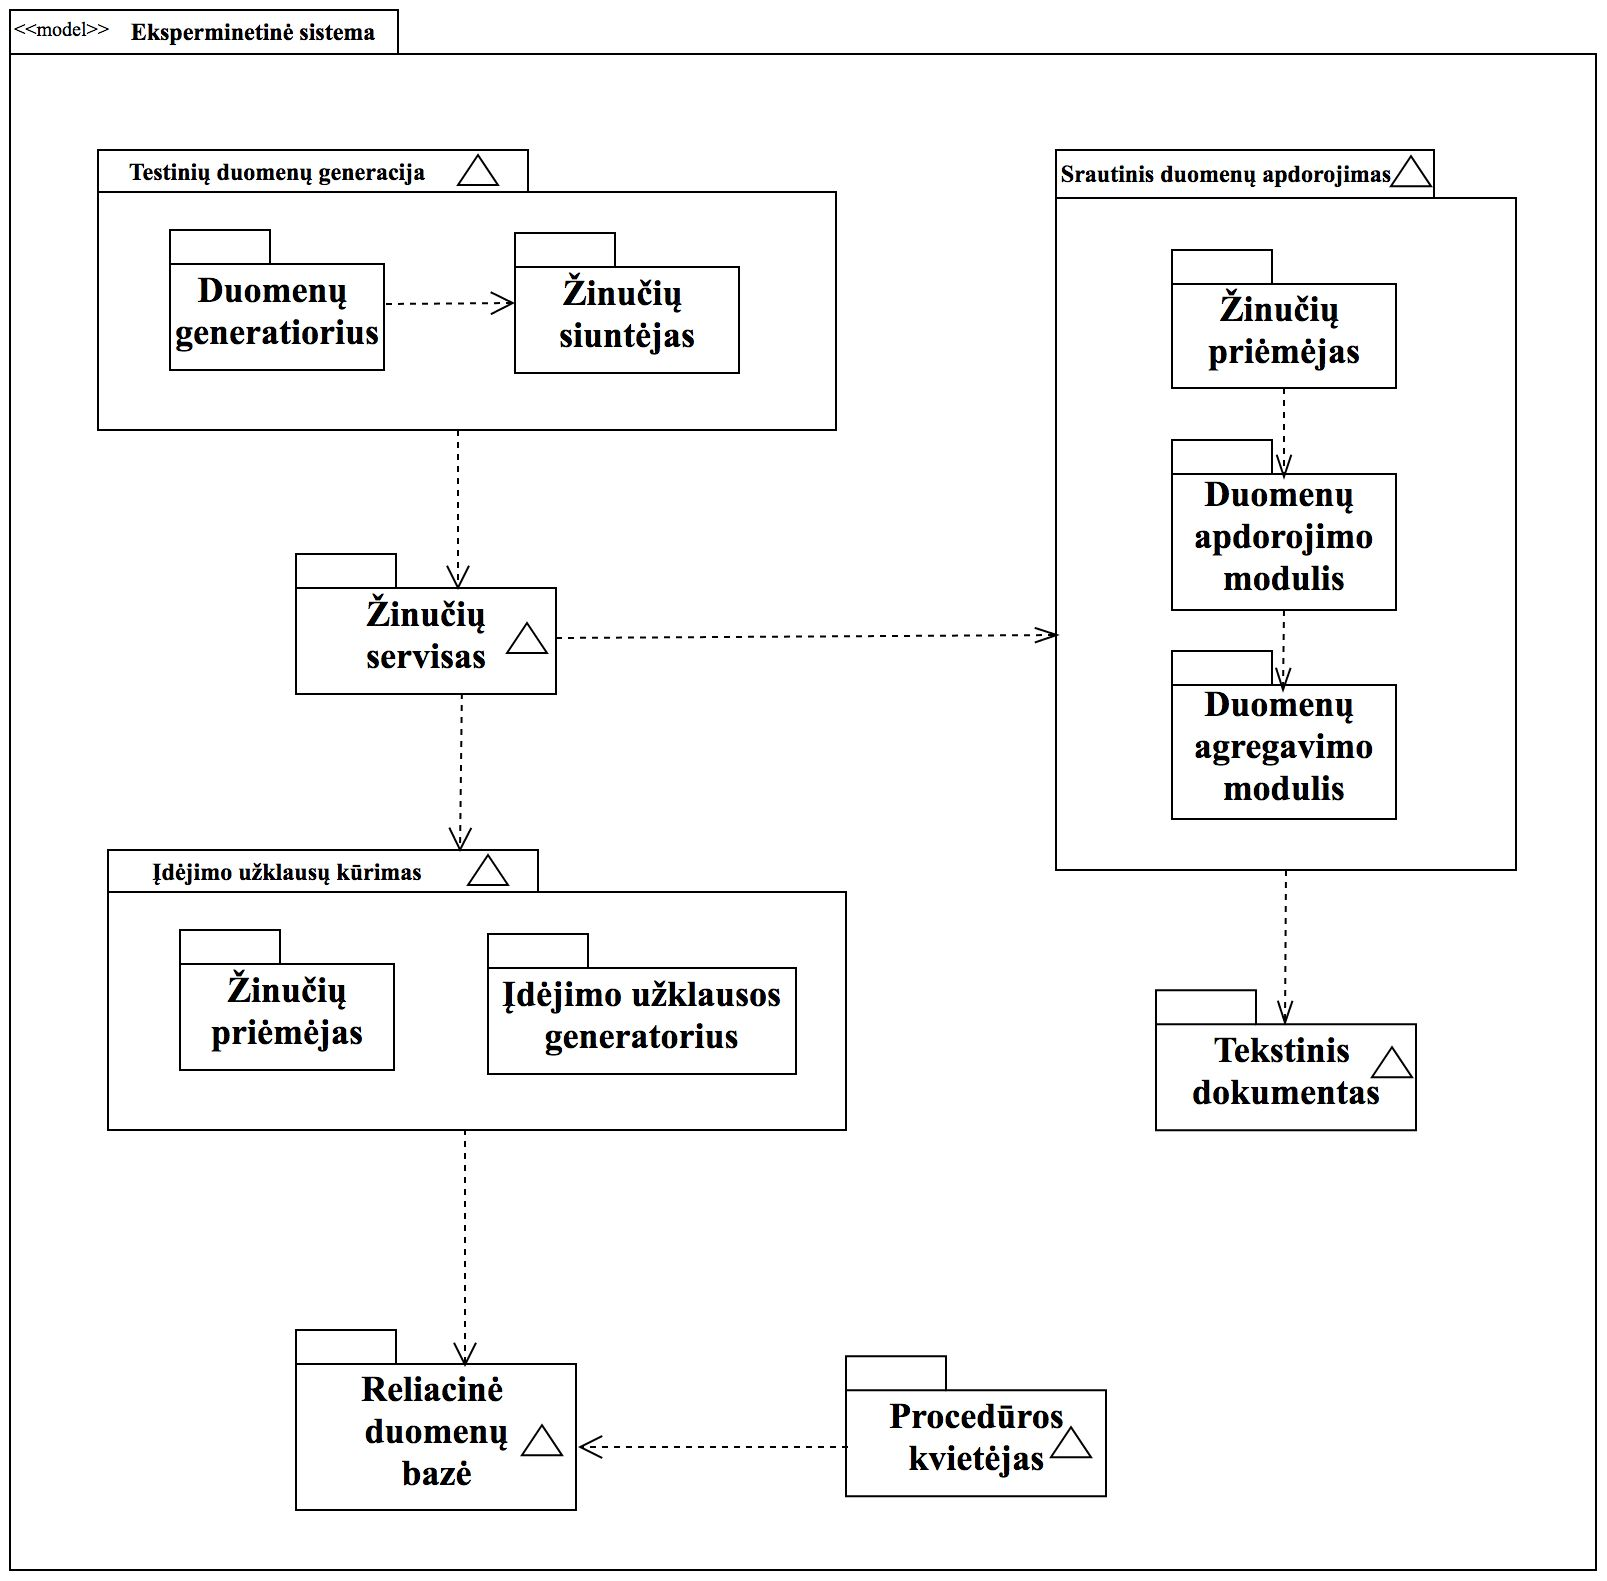
\includegraphics[width=1\textwidth]{img/architecture.jpg}
    \caption{Eksperimentinės sistemos architektūra}
    \label{fig:architecture}
\end{figure}
\subsection{Eksperimento realizacija}


\subsubsection{Testinių duomenų generavimo sprendimo realizacija}

Testinių duomenų generavimo sistema yra sudaryta iš dviejų dalių: ,,Python" kalba parašytas duomenų generatorius ir siuntėjas į žinučių sistemą ir
,,Apache Kafka" žinučių sistema, kuri yra atsakinga už duomenų perdavimą iš generatoriaus į kitus modulius.\par
Su ,,Python" kalba parašytas duomenų generatorius, kuris sukuria nustatytą kiekį duomenų, naudojant ,,random" biblioteką ir, kai apibrėžtas kiekis duomenų sugeneruotas,
 po vieną siunčia į ,,Apache Kafka" žinučių sistemą, naudojant ,,kafka-python" biblioteką. Generuojami duomenys yra pritaikyti skirtingiems sprendimams.
Į srautinio apdorojimo sistemą siunčiami tik duomenys, kuriuos reikia apdoroti ir raktas pagal kurį apdoroti duomenys agreguojami, o į reliacinės duomenų
bazės sprendimą siunčiami tik vienos iš lentelių pirminis raktas, kuris parenkamas atsitiktiniai iš visų įmanomų raktų, ir naujas duomuo. Duomenų siuntimas į 
žinučių sistemą vykdomas nepertraukiamai.  \par

,,Apache Kafka" - tai servisas gaunantis, saugojantis ir siunčiantis duomenis, kurie yra vadinami žinutėmis (angl. messages). Žinutės yra skirstomos pagal temas (angl. topics).
Yra žinučių kūrėjai (angl. producers), kurie siunčia žinutės į tam tikras temas, ir vartotojai (angl. consumers), kurie prenumeruoja (angl. subscribe)
prie temų, kad gautu su jomis susijusias žinutes \cite{thein2014apache}.  Taip pat visos žinutės šia sistema yra perduodamos tekstiniu formatu, 
tam kad bendrauti su ,,Apache Kafka" būtų įmanoma su bet kokia programavimo kalba. Bet dėl to nukenčia greitaveiką kadangi prisideda
papildomas darbas - konvertavimas iš teksto į reikiamą objektą.\par
%,,Apache Kafka" architektūra yra mums aktuali, nes ji laiko visas žinutes savo atmintyje, todėl tą pačią žinutę gali perskaityti keli vartotojai.
Šis testinių duomenų generavimo sprendimas tinka srautinio apdorojimo sprendimams, kadangi ,,Apache Kafka" siunčia žinutes,
kai tik gauna duomenis ir todėl duomenų apdorojimas gali vykti iš karto, o ne tada, kai sistema užklausia. Taip pat ,,Pyhton" programos sugeneruotus duomenis galime
be sunkumų apdoroti su srautinio apdorojimo sprendimu, kuris yra parašytas bet kokia kita programavimo kalba. 
Autoriaus sukurtas reliacinių duomenų bazės sprendimas taip pat naudoja ,,Apache Kafka". Nors ir reliacinės duomenų bazės sprendimo atžvilgiu, ši architektūra yra perteklinė, 
tačiau net pridėjus šį papildomą sluoksnį duomenų įrašymas sulėtėja nežymiai.\par

\subsubsection{Srautinio duomenų apdorojimo sprendimo realizacija}

,,Apache Storm" sistemai kuriama programa yra vadinama topologija (angl. topology), kuri susideda iš ,,Spout" ir ,,Bolt" modulių. ,,Spout" tai modulis gaunantis duomenis
iš išorinės sistemos ir perduodantis juos į pirmą ,,Bolt" modulį. ,,Bolt" yra atsakingi už duomenų apdorojimą ir atidavimą atgal į išorę.
Moduliai tarpusavyje perduoda duomenų ,,Tuple" tipu, kuris laiko duomenis ir architektūros sugeneruotą identifikatorių, 
kurio pagalba užtikrina, kad duomenys sėkmingai nuėjo iki sekančio žingsnio. 
Šiam uždaviniu spręsti buvo pasirinkta sukurti:
\begin{enumerate}
    \item ,,kafka-spout" - ,,Spout" modulis, kuris gauna duomenis iš ,,Apache Kafka" žinučių sistemos ir perduoda juos po jo einančiam ,,Bolt" moduliui.
    \item ,,calculate-price-bolt" - ,,Bolt" modulis, kuris gauna tekstinio tipo duomenis iš ,,kafka-spout" ir apdoroja vieną atėjusį ,,Tuple".
    \item ,,aggregate-price-bolt" - ,,Bolt" modulis, kuris gauna apdorota ,,Tuple" iš ,,calculate-price-bolt" ir įdeda jį į ,,HashMap" tipo sąrašą ir visą sąrašą kas nustatytą laiko tarpą spausdina į tekstinį dokumentą.  
\end{enumerate}\par
Kadangi ,,Apache Storm" yra žemo abstrakcijos lygmens architektūra programuotojas turi pats numatyti paralelizmo lygi kiekviename modulyje. 
Po bandymų buvo nuspręsta modelių konfigūraciją daryti tokią: ,,kafka-spout" - 5 paralelus procesai, ,,calculate-price-bolt"
 - 5 paralelus procesai ir ,,aggregate-price-bolt" - 1 procesas. Paskutinį moduli negalima leisti paraleliai, nes jame saugomas bendras sąrašas,
kurio keitimas iš kelių gijų sugadina duomenis. Srautinio sprendimo greitaveika matuosime:
\begin{enumerate}
    \item Kiek duomenų srautinis sprendimas apdoroja per sekundę.
    \item Kiek užtrunka vieno duomens apdorojimas nuo duomens gavimo iš ,,Apache Kafka" serviso iki gauto duomens agregavimo į bendrą sąrašą pabaigos.
\end{enumerate}

 \subsubsection{Reliacinės duomenų bazės sprendimo realizacija}

Reliacinės duomenų bazės realizavimui buvo pasirinkta ,,Microsoft SQL Server" duomenų bazė, o duomenų apdorojimui parašyta procedūra (angl. stored procedure) ,,GetReports".
Sukurta minimali duomenų bazė, su 3 lentelėmis (\ref{fig:dbdiagram} pav.). Sukurta procedūra ,,GetReports" sujungia šias tris lenteles į vieną, kurioje yra parodoma kiekvienos 
parduotuvės (Shop) uždirbti pinigus pagal nesudėtingą sumavimo formulę.
\begin{figure}[!htbp]
    \centering
    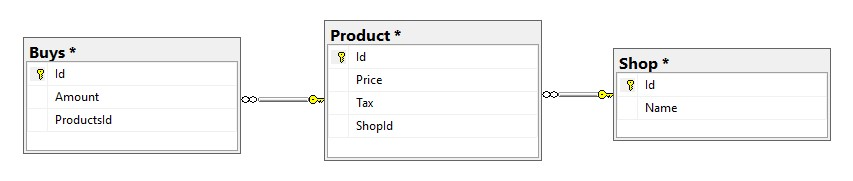
\includegraphics[width=1\textwidth]{img/dbdiagram.jpg}
    \caption{Reliacinė duomenų bazė testavimui}
    \label{fig:dbdiagram}
\end{figure}
Kad duomenys iš generatoriaus patektų į duomenų bazę buvo sukurta programa su ,,Python" kalba kuri gauna duomenis iš ,,Apache Kafka" žinučių sistemos ir talpina jas
duomenų bazėje, kiekviena gauta JSON užkoduota žinutė yra paverčiama į ,,Python" žodyno (angl. dictonary) tipą ir įdedama į įvedimo užklausą, kuri iškarto yra 
įvykdoma duomenų bazėje. Taip užtikrinamas nepertraukiamas duomenų įvedimas į reliacinė duomenų bazę.\par
Procedūros testavimui buvo naudojama papildoma ,,Python" kalba parašyta programa, kuri gavusi žinutę iš ,,Apache Kafka" sistemos sukuria įdėjimo užklausą į duomenų bazę.
Taip pat ,,GetReports" procedūros iškvietimui buvo naudojama ,,Python" kalba parašyta programa, kuri periodiškai kviečia šią procedūrą. 
Kadangi negalima testuoti procedūros taip pat kaip srautinio apdorojimo sprendimą, šis testas bus daromas kitaip.
Vienu metu buvo įvedami nauji duomenys ir tuo pat metu, tam tikru laiko intervalu, kviečiama procedūra ir buvo tikrinama:
    \begin{enumerate}
        \item Kiek duomenų per sekundę galima įdėti į duomenų bazę.
        \item Kiek sekundžių sulėtėja procedūra, kai yra pastoviai įvedami nauji duomenys.
    \end{enumerate}
\subsection{Eksperimento vykdymas}
Kompiuterio komponentų ir programų versijų su kuriais buvo vykdomas eksperimentas specifikacijos (\ref{table:hardware} lentelė).
\begin{table}[!htbp]
    \begin{center}
        \caption{Įrangos specifikacija}
        \label{table:hardware}
        \begin{tabular}{ | l | l |  } 
            \hline
            Procesorius & Intel i7-7700k 4,5 GHz \\* \hline
            Operatyvioji atmintis & 16 GB - 2666 Mhz \\* \hline
            Ilgalaikė atmintis & SSD 512 GB \\* \hline
            Operacinė sistema & Windows 10 64bit \\* \hline
            Reliacinė duomenų bazė & Windows SQL Server 14 \\* \hline
            Srautinio apdorojimo architektūra & Apache Storm 1.2.2 \\* \hline
            Žinučių sistema & Apache Kafka 1.1.0 \\* \hline
        \end{tabular}
    \end{center}
\end{table}\par

\subsubsection{Reliacinės duomenų bazės sprendimo eksperimento vykdymas}
Į pradinę duomenų bazę buvo įrašyti: 2,000 parduotuvių (Shop), kurios turi 0 arba daugiau prekių, 1,000,000 prekių (Product), kurios turi 0 arba daugiau pirkimų ir 10,000,000 pirkimų (Buys).
Prieš pradedant eksperimentą buvo išmatuota, kiek užtrunka ,,GetReports" procedūra, neapkraunant duomenų bazės kitais veiksmais, ir kiek laiko užtrunka visų duomenų įdėjimas,
nedarant kitų užklausų. 
Eksperimento eiga su reliacine duomenų bazės sprendimu:
\begin{enumerate} 
\item Paleidžiama ,,Python" programa gaunanti žinutes iš ,,Apache Kafka" žinučių sistemos ir įvedanti tuos duomenis į duomenų bazę. 
\item Paleidžiama programa kviečianti procedūrą ,,GetReports" ir nustatyta, kad ji procedūrą kviestų kas 5 sekundes norint simuliuoti realią apkrovą,
po kiekvieno kvietimo ji fiksuoja kiek laiko užtrūko ir kelintą kartą ji yra kviečiama. 
\item Paleidžiamas testinių duomenų generatorius.
\end{enumerate}
\subsubsection{Srautinio duomenų apdorojimo sprendimo eksperimento vykdymas}

Prieš pradedant testavimą į sistemą buvo sugeneruoti 10,000,000 įrašų, kad būtų sudarytos sąlygos panašios kaip ir reliacinės duomenų bazės.
Šiai sistemai pagal nutylėjimą buvo išskirti 832 megabaitai operatyvios atminties (angl. RAM). 
Eksperimento eiga su srautinio duomenų apdorojimo sprendimu:
\begin{enumerate} 
\item Paleidžiama ,,Apache Storm" sistema ir į ją užkraunama sukurta topologija.
\item Paleidžiamas testinių duomenų generatorius.
\end{enumerate}
\newpage
\subsection{Eksperimento rezultatai}
\begin{table}[!htbp]
    \begin{center}
        \caption{Rezultatai}
        \label{table:results}
        \begin{tabular}{ | l | p{4cm} | p{3cm} | } 
            \hline
              & Reliacinės duomenų bazės sprendimas & Srautinio apdorojimo sprendimas \\* \hline
            Pralaidumas (duomenų kiekis per sekundę) & \textasciitilde4,200 & \textasciitilde5,475 \\* \hline
            Vienos duomens apdorojimas ir agregavimas  & \textasciitilde12 sekundžių & \textasciitilde75 milisekundės\\* \hline
        \end{tabular}
    \end{center}
\end{table}\par
\subsubsection{Reliacinės duomenų bazės sprendimo eksperimento rezultatai}
Tiesiog kviečiama procedūrą ,,GetReports" trunka vidutiniškai 12 sekundžių. Leidžiant įdėjimo užklausas, be jokios kitos apkrovos ant duomenų bazės, 1,5 milijonų duomenų
buvo įdėti per 358 sekundžių, beveik 6 minutes. Tačiau paleidus tokį pat pastovų įrašų srautą į duomenų bazę ir bandant tuo pačiu metu gauti apdorotus duomenis,
procedūra užtruko vidutiniškai 29 sekundes ir taip pat apdorotas duomenų sąrašas po generavimo atsiliko virš 120,000 įrašų - tiek duomenų buvo įdėta procedūros veikimo metu. 
Per visą naujų duomenų įdėjimo laiką procedūra ,,GetReports" buvo ivykdyta 10 kartų.
Taip pat vienas iš procedūros trūkumų - įdėjus bent vieną naują duomenį ir norint gauti ataskaitą turi iš naujo būti vykdoma procedūra, kurios trukmė, kai nėra 
paleista jokia kita užklausa, apie 12 sekundžių su testuojama duomenu imtimi.

\subsubsection{Srautinio duomenų apdorojimo sprendimo eksperimento rezultatai}
Paleista testavimo programa siunčianti 1,5 milijono duomenų neribojant siuntimo greičio, rezultatai buvo stebimi įrašais tekstiniame dokumente.
Visi, 1,5 milijonų, duomenų buvo apdoroti per 274 sekundes, tai yra maždaug 4,5 minutės. Vidutiniška vienos operacijos trukmė nuo 
patekimo į ,,Apache Kafka" žinučių sistemą iki galutinio pridėjimo prie bendro sąrašo - 75 milisekundės.
Lėčiausia sistemos grandis buvo ,,aggregate-price-bolt", nes jo negalima buvo leisti paraleliai. Šios sistemos veikimą pagreitinti 
įmanoma tik perdavus paskutinio moduliu agregavimą į sąrašą kitai architektūrai, kadangi visus kitus veiksmus galima leisti paraleliai.

\sectionnonum{Rezultatai ir išvados}

\textbf{Darbo rezultatai:}
\vspace{1 mm}

    \begin{enumerate}
        \item Sukurtas testinių duomenų generatorius - \uri{https://git.mif.vu.lt/vyzi2849/test-data-generator-python}, 
        sukurtas supaprastinto uždavinio sprendimas su reliacine duomenų baze - \uri{https://git.mif.vu.lt/vyzi2849/database-testing-tools-python}
         ir su pasirinkta srautinio apdorojimo architektūra - \uri{https://git.mif.vu.lt/vyzi2849/storm-topology-java}.
        \item Uždavinio sprendimai palyginti pagal pralaidumo testų rezultatus.
    \end{enumerate}
    \vspace{1 mm}

\textbf{Išvados:}
\vspace{1 mm}

    \begin{enumerate}
    \item Eksperimento būdu pagrįsta, kad siūloma sistema gali būti įgyvendinama.
    \item Pralaidumo testavimo metu įrodyta, kad srautinio duomenų apdorojimo sprendimas duomenis išskaičiuoja 
    agreguotas rodiklio reikšmes greičiau (75 milisekundės) nei reliacinių duomenų bazės sprendimas (12 sekundžių) 
    ir srautinio apdorojimo sprendimas nėra priklausomas nuo kitų tuo pačiu metu vykdomų procesų.
    \item Eksperimentui sukurtos sistemos srautinio duomenų apdorojimo sprendimo pralaidumas aukštesnis 
    (\textasciitilde5,475 duomenų per sekundę), negu reliacinės duomenų bazės (\textasciitilde 4,200 duomenų per sekundę). 
    \item Srautinio apdorojimo architektūra ,,Apache Storm" šiam uždaviniui užtikrina duomenų apdorojimą milisekundžių greičiu,
    kadangi suagreguotos reikšmės laikomos operatyvioi atmintyje ir nauji apdoroti duomenis yra pridedami prie jau esamo sąrašo.

    \end{enumerate}

\printbibliography[heading=bibintoc] 

\end{document}
